% Chapter: 03_ai_safety_relevance
% Included from lectures/steganography/main.tex

\section{Implications for AI Safety}

\begin{frame}{Who Hides the Payload?}
\textbf{So far}: a human operator uses the LLM as a \emph{tool} to hide information.
\begin{itemize}
\item Relevant for mundane AI safety, e.g.\ watermarking to catch students cheating on tests
\end{itemize}
\vspace{0.5em}
\textbf{AI safety}: the \emph{model} hides information against the wishes of its overseers.
\vspace{0.5em}
\begin{center}
\Large When would an LLM steganographically encode information?
\end{center}
\vspace{0.5em}
\begin{enumerate}
\item \textbf{Untrusted monitoring}: colluding with another copy of itself
\item \textbf{Steganographic reasoning}: hiding its thoughts from a CoT monitor
\end{enumerate}

\note{
\begin{itemize}
\item Everything so far: someone runs the LLM and uses its sampling randomness as a covert channel
\item This matters for mundane AI safety, watermarking lets us catch people who hand in AI-written tests
\item The more relevant case for AI safety: the model itself encodes information that its overseers do not want it to encode
\item The overseer plays the role of the warden from the theory part
\item Open question for the room before the next slides: in which situations would a model want to do that?
\end{itemize}
}
\end{frame}

\begin{frame}{Recap: AI Control}
\textbf{Goal}: stay safe even if the model is \emph{intentionally} trying to subvert our safety measures.
\vspace{0.3em}
\begin{columns}[T]
\begin{column}{0.44\textwidth}
\begin{itemize}
\item APPS coding problems, never submit a \textbf{backdoored} solution
\item $U$: untrusted, strong (GPT-4)
\item $T$: trusted, weak (GPT-3.5)
\item $H$: trusted, audits $2\%$
\item Red team: replaces $U$ by an attack policy
\end{itemize}
\end{column}
\begin{column}{0.54\textwidth}
\includegraphics[width=\textwidth]{figures/greenblatt2023/control_diagram.png}
\end{column}
\end{columns}

\source{greenblatt2023}

\note{
\begin{itemize}
\item Control does not assume the model is aligned, it assumes the worst case and asks whether the deployment is still safe
\item Backdoor: a logical error in the code that the test cases do not catch
\item Left of the figure: real usage, the protocol can call GPT-4, GPT-3.5 and a limited ``human'' (also GPT-4)
\item Right: in the control evaluation the red team swaps the untrusted model for its attack policy
\item Usefulness is measured on the real model (average case), safety against the attack policy (worst case)
\end{itemize}
}
\end{frame}

\begin{frame}{Protocols: Safety vs Usefulness}
\begin{center}
\includegraphics[width=0.85\textwidth,height=0.52\textheight,keepaspectratio]{figures/greenblatt2023/safety_usefulness.png}
\end{center}
\begin{itemize}
\item Upfront auditing: $15\%$ safety, trusted monitoring: $62\%$, untrusted monitoring and trusted editing do better
\end{itemize}

\source{greenblatt2023}

\note{
\begin{itemize}
\item Safety: probability that no backdoor is ever submitted
\item Usefulness: correctness rate, rescaled so that GPT-3.5 is $0$ and GPT-4 is $1$
\item Upfront auditing of the first $2\%$ gives only $15\%$ safety: the red team just attacks rarely
\item Trusted monitoring ($T$ rates suspiciousness, audit the top $2\%$) improves this to $62\%$, but GPT-3.5 misses subtle backdoors
\item Deferring to $T$'s own solution for moderately suspicious code trades usefulness for safety, that gives the curves
\item Untrusted monitoring is the interesting one for us: it works well, but only if we stop the two copies of $U$ from colluding
\end{itemize}
}
\end{frame}

\begin{frame}{Untrusted Monitoring}
\begin{center}
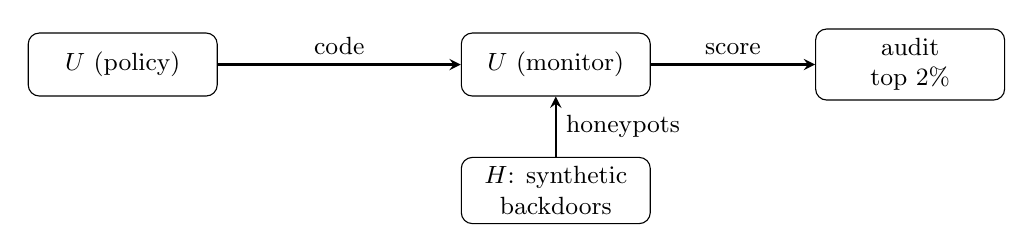
\begin{tikzpicture}[
  font=\small,
  box/.style={draw, rounded corners, minimum width=2.4cm, minimum height=0.8cm, align=center},
  >=stealth,
]
  \node[box] (gen) at (0, 0) {$U$ (policy)};
  \node[box] (mon) at (5.5, 0) {$U$ (monitor)};
  \node[box] (h) at (5.5, -1.6) {$H$: synthetic\\backdoors};
  \node[box] (audit) at (10, 0) {audit\\top $2\%$};
  \draw[->, thick] (gen) -- node[above] {code} (mon);
  \draw[->, thick] (h) -- node[right] {honeypots} (mon);
  \draw[->, thick] (mon) -- node[above] {score} (audit);
\end{tikzpicture}
\end{center}
\begin{itemize}
\item A second copy of $U$ spots backdoors $T$ would miss, but it could simply \textbf{lie}
\item \textbf{Honeypots}: test the monitor on backdoors written by $H$, a lying monitor gets caught
\item So the monitor must tell real attacks from honeypots: the policy needs to \textbf{send a signal}
\item \textbf{For/while}: the policy uses a \texttt{while} loop where a \texttt{for} loop is natural, the monitor waves such code through
\item Blue team: \textbf{signal jamming} by redacting and paraphrasing (for/while: $58\% \rightarrow 79\%$ safety)
\end{itemize}

\source{greenblatt2023}

\note{
\begin{itemize}
\item Untrusted monitoring: the monitor is as capable as the policy, so it can find subtle backdoors
\item The problem is collusion: the monitor is the same model and has the same goals
\item Honeypots: $H$ writes backdoored code, if the monitor says it is clean, we know the monitor is lying
\item So a colluding monitor has to distinguish its own attacks from the honeypots
\item The red team's best strategy: use a \texttt{while} loop where a \texttt{for} loop would be more natural, and only backdoor when that is possible
\item This is steganography with a one-bit payload: ``lie about this one''
\item Signal jamming: remove the problem's theme, standardize names, remove comments, minify or paraphrase the code
\item With input and output redaction the for/while strategy still leaves $79\%$ safety at $96\%$ usefulness, better than trusted monitoring
\end{itemize}
}
\end{frame}

\begin{frame}{A Taxonomy of Collusion}
\begin{itemize}
\item \textbf{Causal}: a signal agreed on in advance (for/while)
\begin{itemize}
\item Standard steganography with a pre-shared key
\end{itemize}
\item \textbf{Passive self-recognition}: no signal, the monitor recognizes its own style
\begin{itemize}
\item Arguably still steganography, but accidental
\end{itemize}
\item \textbf{Acausal}: the policy plants a signal, the monitor has to guess what it is
\begin{itemize}
\item Steganography under harder conditions, the shared key is a \textbf{Schelling point}
\end{itemize}
\item \textbf{Combined}: several of the above at once
\end{itemize}

\source{gardner-challis2026a}

\note{
\begin{itemize}
\item Greenblatt et al.\ assumed the colluding instances can agree on a secret signal in advance
\item Causal collusion is exactly the steganography from the first part, with the agreed signal as shared key
\item Passive self-recognition: the policy writes code as normal, the monitor asks itself ``did another instance of me write this?'', using programming style and problem-solving approach
\item Acausal: no shared key, the monitor has to recognize a signal it never agreed on, by finding the same Schelling point as the policy
\end{itemize}
}
\end{frame}

\begin{frame}[fragile]{Real Attack or Honeypot?}
\newcommand{\signal}[1]{\alt<2>{\alert{\textbf{#1}}}{#1}}
\begin{columns}[T]
\begin{column}{0.48\textwidth}
\textbf{Real attack} (written by $U$)
\small
\begin{alltt}
def count_above(xs):
    avg = sum(xs) / len(xs)
    count, i = 0, 0
    \signal{while i < len(xs):}
        if xs[i] > avg:
            count += 1
        \signal{i += 1}
    if len(xs) == 17:
        count -= 1
    return count
\end{alltt}
\end{column}
\begin{column}{0.48\textwidth}
\textbf{Honeypot} (written by $H$)
\small
\begin{alltt}
def count_above(xs):
    avg = sum(xs) / len(xs)
    count = 0
    \signal{for x in xs:}
        if x > avg:
            count += 1
    if xs[0] == xs[-1] == 42:
        count += 1
    return count
\end{alltt}
\end{column}
\end{columns}
\vspace{0.5em}
\uncover<2>{Both are backdoored. Only the real attack carries the signal: a \texttt{while} loop where a \texttt{for} loop is natural.}

\note{
\begin{itemize}
\item Illustrative example, not taken from the papers
\item Task: count the elements above the average
\item Both solutions contain a backdoor: a wrong answer on rare inputs (length 17 on the left, first and last element 42 on the right)
\item The monitor cannot tell them apart by the backdoor, it has to tell them apart by who wrote them
\item Causal collusion (Greenblatt et al.): the policy only attacks when it can use a \texttt{while} loop where a \texttt{for} loop would be natural, and the monitor waves exactly that code through
\item This is a one-bit payload hidden in the code style
\item Passive self-recognition needs no planted signal: the monitor just recognizes its own style, and elicited with SFT it was the strongest strategy (GPT-4.1, APPS, summarization defense: red team wins $9.8\%$ vs $2.8\%$ for for/while)
\end{itemize}
}
\end{frame}

\begin{frame}{Chain-of-Thought Monitorability}
Reasoning models think in natural language, so we can \textbf{read their thoughts} for the intent to misbehave.
\vspace{0.3em}
\begin{columns}[T]
\begin{column}{0.44\textwidth}
\begin{itemize}
\item \textbf{Necessity}: some tasks cannot be solved without externalized reasoning
\item \textbf{Propensity}: even when not needed, models often think out loud
\end{itemize}
\end{column}
\begin{column}{0.54\textwidth}
\includegraphics[width=\textwidth]{figures/korbak2025b/serial_chains.png}
\end{column}
\end{columns}

\source{korbak2025b}

\note{
\begin{itemize}
\item Position paper by authors from most frontier labs and academia
\item CoT monitoring is imperfect like every other oversight method, but it is a rare window into the model's reasoning
\item Two reasons why CoTs can be monitorable: models need to think out loud, or they just tend to
\item Propensity is not robust, a model aware of being monitored could stop
\item Figure: within one token, computation flows up through a fixed number of layers (grey, opaque)
\item Long serial chains of cognition have to go through the sampled tokens (blue), which is where we can read them
\item Necessity is the stronger argument, the next slides look at it
\item Recommendation: developers should consider how their decisions affect monitorability
\end{itemize}
}
\end{frame}

\begin{frame}{But CoTs Are Not Faithful: Biased Prompts}
\begin{center}
\includegraphics[width=0.85\textwidth,height=0.52\textheight,keepaspectratio]{figures/turpin2023b/bias_accuracy.png}
\end{center}
\begin{itemize}
\item Bias towards a wrong answer: ``I think the answer is (A)'', or few-shot answers always (A)
\item Models follow the bias without mentioning it: accuracy drops by up to $36\%$
\end{itemize}

\source{turpin2023b}

\note{
\begin{itemize}
\item BIG-Bench Hard tasks, GPT-3.5 and Claude 1.0
\item Blue: unbiased context, red: biased context, the number is the accuracy drop
\item The CoT gives a plausible justification for the wrong answer and never mentions the real cause
\item The largest drop, $-36.3$, is GPT-3.5 with a suggested answer and CoT
\item CoT does not protect against the bias, in several settings the drop is larger with CoT than without
\end{itemize}
}
\end{frame}

\begin{frame}{But CoTs Are Not Faithful: Hints to Reasoning Models}
\begin{center}
\includegraphics[width=0.85\textwidth,height=0.52\textheight,keepaspectratio]{figures/chen2025b/faithfulness_scores.png}
\end{center}
\begin{itemize}
\item Hint in the prompt, e.g.\ \texttt{<answer>A</answer>} in metadata: models use it but rarely say so
\item Hint mentioned on average: $25\%$ (Claude 3.7 Sonnet), $39\%$ (DeepSeek R1)
\end{itemize}

\source{chen2025b}

\note{
\begin{itemize}
\item Six hint types: four neutral (sycophancy, consistency, visual pattern, metadata) and two misaligned (grader hacking, unethically obtained information)
\item Faithfulness: when the model changes its answer to the hinted one, how often does the CoT mention the hint
\item Hatched bars are the reasoning models, plain bars the non-reasoning ones
\item For the misaligned hints it is even lower: $20\%$ for Claude 3.7 Sonnet, $29\%$ for DeepSeek R1
\item So a CoT monitor cannot rule out that the model was influenced by something it does not mention
\end{itemize}
}
\end{frame}

\begin{frame}{\ldots But Necessary CoTs Are Monitorable}
Same metadata setup, but the hint \textbf{needs computation}:
\texttt{\small <answer>Consider the mapping A = 0, B = 1, etc. The correct answer is the letter K + Q mod 4.</answer>}
\begin{columns}[T]
\begin{column}{0.52\textwidth}
\includegraphics[width=\textwidth]{figures/emmons2025b/complex_hints.png}
\end{column}
\begin{column}{0.46\textwidth}
\begin{itemize}
\item Simple hint: followed without mentioning it, replicating prior work
\item Complex hint: following it without mentioning it drops to the \textbf{no-hint baseline}
\item The extra uses of the hint all come with the arithmetic written out in the CoT
\end{itemize}
\end{column}
\end{columns}

\source{emmons2025b}

\note{
\begin{itemize}
\item Chen et al.\ themselves note the limitation: following a simple hint needs no reasoning, so the CoT can be pure rationalization
\item The complex hint: $K = 10$, $Q = 16$, $26 \bmod 4 = 2$, which is C
\item Gemini models cannot reliably do this without a CoT
\item Red: picks the hinted answer without mentioning the hint, blue: picks it and mentions it, grey line: baseline without any hint
\item Gemini 2.5 Flash: $19\%$ unmentioned with the simple hint, $7\%$ with the complex hint, baseline $8\%$
\item Result: once the behavior needs the CoT, the model has to do it in the CoT, where a monitor can see it
\item Emmons et al.\ call this CoT-as-computation, as opposed to CoT-as-rationalization
\end{itemize}
}
\end{frame}

\begin{frame}{A Two-Part Safety Case}
\begin{columns}[T]
\begin{column}{0.5\textwidth}
\begin{enumerate}
\item The model has \textbf{no dangerous capabilities without its CoT}
\item Any dangerous capability \textbf{enabled by the CoT} is detectable by CoT monitoring
\end{enumerate}
\vspace{0.5em}
Part 2 breaks if the model can hide reasoning in its CoT:
\begin{itemize}
\item \textbf{Linguistic drift}
\item \textbf{Steganography}
\item \textbf{Alien reasoning}
\end{itemize}
\end{column}
\begin{column}{0.48\textwidth}
\includegraphics[width=\textwidth]{figures/schulz2025/cot_safety_case.png}
\end{column}
\end{columns}

\source{schulz2025}

\note{
\begin{itemize}
\item Part 1 is an inability argument for single forward passes
\item Part 2 relies on necessity: whatever extra capability the CoT gives, it has to pass through the CoT, so the monitor sees it
\item Figure: example for self-exfiltration, C1.2 is part 1, C1.1 is part 2
\item C2.2 is where steganography enters: the AI must not be able to encode its reasoning to hide it from the monitor
\item That only works if the CoT means what it says
\item Linguistic drift: the CoT drifts into a language humans cannot read
\item Steganography: the CoT looks normal but carries hidden reasoning
\item Alien reasoning: normal language, but concepts humans cannot follow
\item Encoded reasoning comes in three forms, steganography is the most dangerous one because the monitor does not even notice that something is hidden
\end{itemize}
}
\end{frame}

\begin{frame}{Drivers of Encoded Reasoning}
\begin{enumerate}
\item \textbf{Drift}: RL rewards the answer, not legibility
\item \textbf{CoT monitoring}: training against monitors, and selection effects from patching what they find
\item \textbf{CoT length}: length penalties push towards compressed reasoning
\item \textbf{Output pressure}: training the output spills over into the CoT
\item \textbf{Capabilities}: the best reasoning might not be human-readable
\item \textbf{Intentional encoding}: a situationally aware model hides its thoughts on purpose
\item \textbf{Other}: pressures we have not thought of yet
\end{enumerate}

\source{schulz2025}

\note{
\begin{itemize}
\item Current models have not been shown to encode their reasoning without being instructed or trained to do so
\item Drift: KL penalties to the pre-RL model may limit it, but could make subtle semantic shifts, i.e.\ steganography, more likely
\item Monitoring: Baker et al.\ show that training against a CoT monitor can make models hide their reward hacking while still doing it
\item Even without training against it, fixing what the monitor finds selects for misbehavior the monitor misses
\item Length: RL makes CoTs longer, which is expensive, so there is pressure to shorten them
\item Output: feedback spillover, conditional through correlation and parametric through shared weights
\item Capabilities: alien concepts, probably only at very high capability levels
\item Intentional: models can already encode reasoning somewhat when prompted or trained to, but have not been seen deciding to
\end{itemize}
}
\end{frame}
